\documentclass[fleqn,10pt]{SelfArx} % Document font size and equations flushed left

\usepackage[english]{babel} % Specify a different language here - english by default

\usepackage{lipsum} % Required to insert dummy text. To be removed otherwise
\usepackage{xcolor} % Required for specifying custom colours
\usepackage[T1]{fontenc}
\usepackage{tgtermes}
%\definecolor{grey}{rgb}{0.9,0.9,0.9} % Colour of the box surrounding the title
\usepackage{multicol}
\usepackage{graphicx}
\usepackage{placeins}
\usepackage{longtable}
%----------------------------------------------------------------------------------------
%	COLUMNS
%----------------------------------------------------------------------------------------

\setlength{\columnsep}{0.55cm} % Distance between the two columns of text
\setlength{\fboxrule}{0.75pt} % Width of the border around the abstract

%----------------------------------------------------------------------------------------
%	COLORS
%----------------------------------------------------------------------------------------

\definecolor{color1}{RGB}{0,0,0} % Color of the article title and sections
\definecolor{color2}{rgb}{0.97, 0.97, 1.0}
%\definecolor{color2}{RGB}{0,0,0}
%\definecolor{color2}{RGB}{0,20,20} % Color of the boxes behind the abstract and headings

%----------------------------------------------------------------------------------------
%	HYPERLINKS
%----------------------------------------------------------------------------------------

\usepackage{hyperref} % Required for hyperlinks

%\hypersetup{
%	hidelinks,
%	colorlinks,
%	breaklinks=true,
%	urlcolor=color2,
%	citecolor=color1,
%	linkcolor=color1,
%	bookmarksopen=false,
%	pdftitle={Title},
%	pdfauthor={Author},
%}
\hypersetup{
    colorlinks=true,
    linkcolor=black,
    filecolor=magenta,      
    urlcolor=cyan,
}

%----------------------------------------------------------------------------------------
%	ARTICLE INFORMATION
%----------------------------------------------------------------------------------------

%\JournalInfo{foo} % Journal information
%\Archive{} % Additional notes (e.g. copyright, DOI, review/research article)
 \lhead{
\includegraphics[width=3cm]{rs_logo}}

\PaperTitle{JTAG-to-AXI IP} % Article title

\Authors{ } % Authors
%\Authors{Zafar Ali} % Authors

%\affiliation{\textsuperscript{1}\textit{Department of Biology, University of Examples, London, United Kingdom}} % Author affiliation
%\affiliation{\textsuperscript{2}\textit{Department of Chemistry, University of Examples, London, United Kingdom}} % Author affiliation
%\affiliation{*\textbf{Corresponding author}: john@smith.com} % Corresponding author

%\Keywords{Keyword1 --- Keyword2 --- Keyword3} % Keywords - if you don't want any simply remove all the text between the curly brackets
\Keywords{} % Keywords - if you don't want any simply remove all the text between the curly brackets
\newcommand{\keywordname}{Keywords} % Defines the keywords heading name

%----------------------------------------------------------------------------------------

%----------------------------------------------------------------------------------------

\begin{document}


\begin{titlepage} % Suppresses displaying the page number on the title page and the subsequent page counts as page 1


	\fontsize{30pt}{40pt}\selectfont
	\noindent JTAG to AXI IP \\
	\vfill % Space between the title box and author information
	
	\begin{multicols}{2}
		\raggedright% Right align the text
		\fontsize{10pt}{20pt}\selectfont
		Specification Document v0.01 \\ \textbf{Release:} \text{October 10, 2022}

		\columnbreak
		\raggedleft % Right align the text
		
\includegraphics[width=4cm]{rs_logo}\\
	\end{multicols}
\end{titlepage}

%\maketitle % Output the title and abstract box
\tableofcontents % Output the contents section
%\thispagestyle{empty} % Removes page numbering from the first page

%----------------------------------------------------------------------------------------
%	ARTICLE CONTENTS
%----------------------------------------------------------------------------------------

\newpage
%\begin{multicols}{2}

%\addcontentsline{toc}{section{}}{{tocdepth}{3}} % Adds this section to the table of contents
\section{JTAG to AXI IP} % The \section*{} command stops section numbering
\subsection{Introduction}
\vskip 1mm
\paragraph{}
The JTAG-to-AXI IP is an AXI-compliant IP that can be used to initiate AXI4 transactions inside the FPGA. The IP provides an AXI4 master interface on one side and a JTAG interface on the other side. The IP is most suited for use in debugging of AXI-compliant IP cores and can send test vectors to AXI4 memory mapped slaves in order to verify their functionality. The IP implements standard 1- bit Bypass, 32-bit ID and 5-bit Instruction registers. Other than the standard registers, the IP also provides two user registers which can be used to send and receive data from AXI slaves.\\
\noindent
%----------------------------------------------------------------------------------------\\
%TODO: \\
%----------------------------------------------------------------------------------------
\\
%\lipsum[1-3] % Dummy text
% and some mathematics $\cos\pi=-1$ and $\alpha$ in the text\footnote{And some mathematics $\cos\pi=-1$ and $\alpha$ in the text.}.
%\columnbreak

\subsection{Features}
\vskip 1mm
The JTAG-to-AXI IP provides the following features to the user:
\hskip 2mm
\begin{itemize}[noitemsep]
    \item AXI4 master interface for integration with logic modules.
	\item Configurable data width of AXI4 bus (32/64 bits).
	\item Dedicated 96 bits wide AXI data-in register.
	\item Dedicated 64 bits wide AXI data-out register.
\end{itemize}

\subsection{Resource Utilization}
\begin{table}[h]
	\resizebox{\textwidth}{!}{%
		\begin{tabular}{|l|l|l|l|}
			\hline
			\textbf{Configuration} & \textbf{FPGA} & \textbf{Resources}                       & \textbf{Description}                            \\ \hline
			Minimum Resource       & Gemini        & LUTS= ??, FLOPS = ??, BRAM = ??, DSP =?? & Configured for 32-bit wide AXI-bus                    \\ \hline
			Maximum Resource       & Gemini        & LUTS= ??, FLOPS = ??, BRAM = ??, DSP =?? & Configured for 64-bit wide AXI-bus            \\ \hline
		\end{tabular}%
	}
	\caption{Raptor Report}
	\label{tab:table-1}
\end{table}

\section{Functional Description}

\subsection{JTAG Boundary Scan Register}
\begin{figure}[!ht]\centering % Using \begin{figure*} makes the figure take up the entire width of the page
	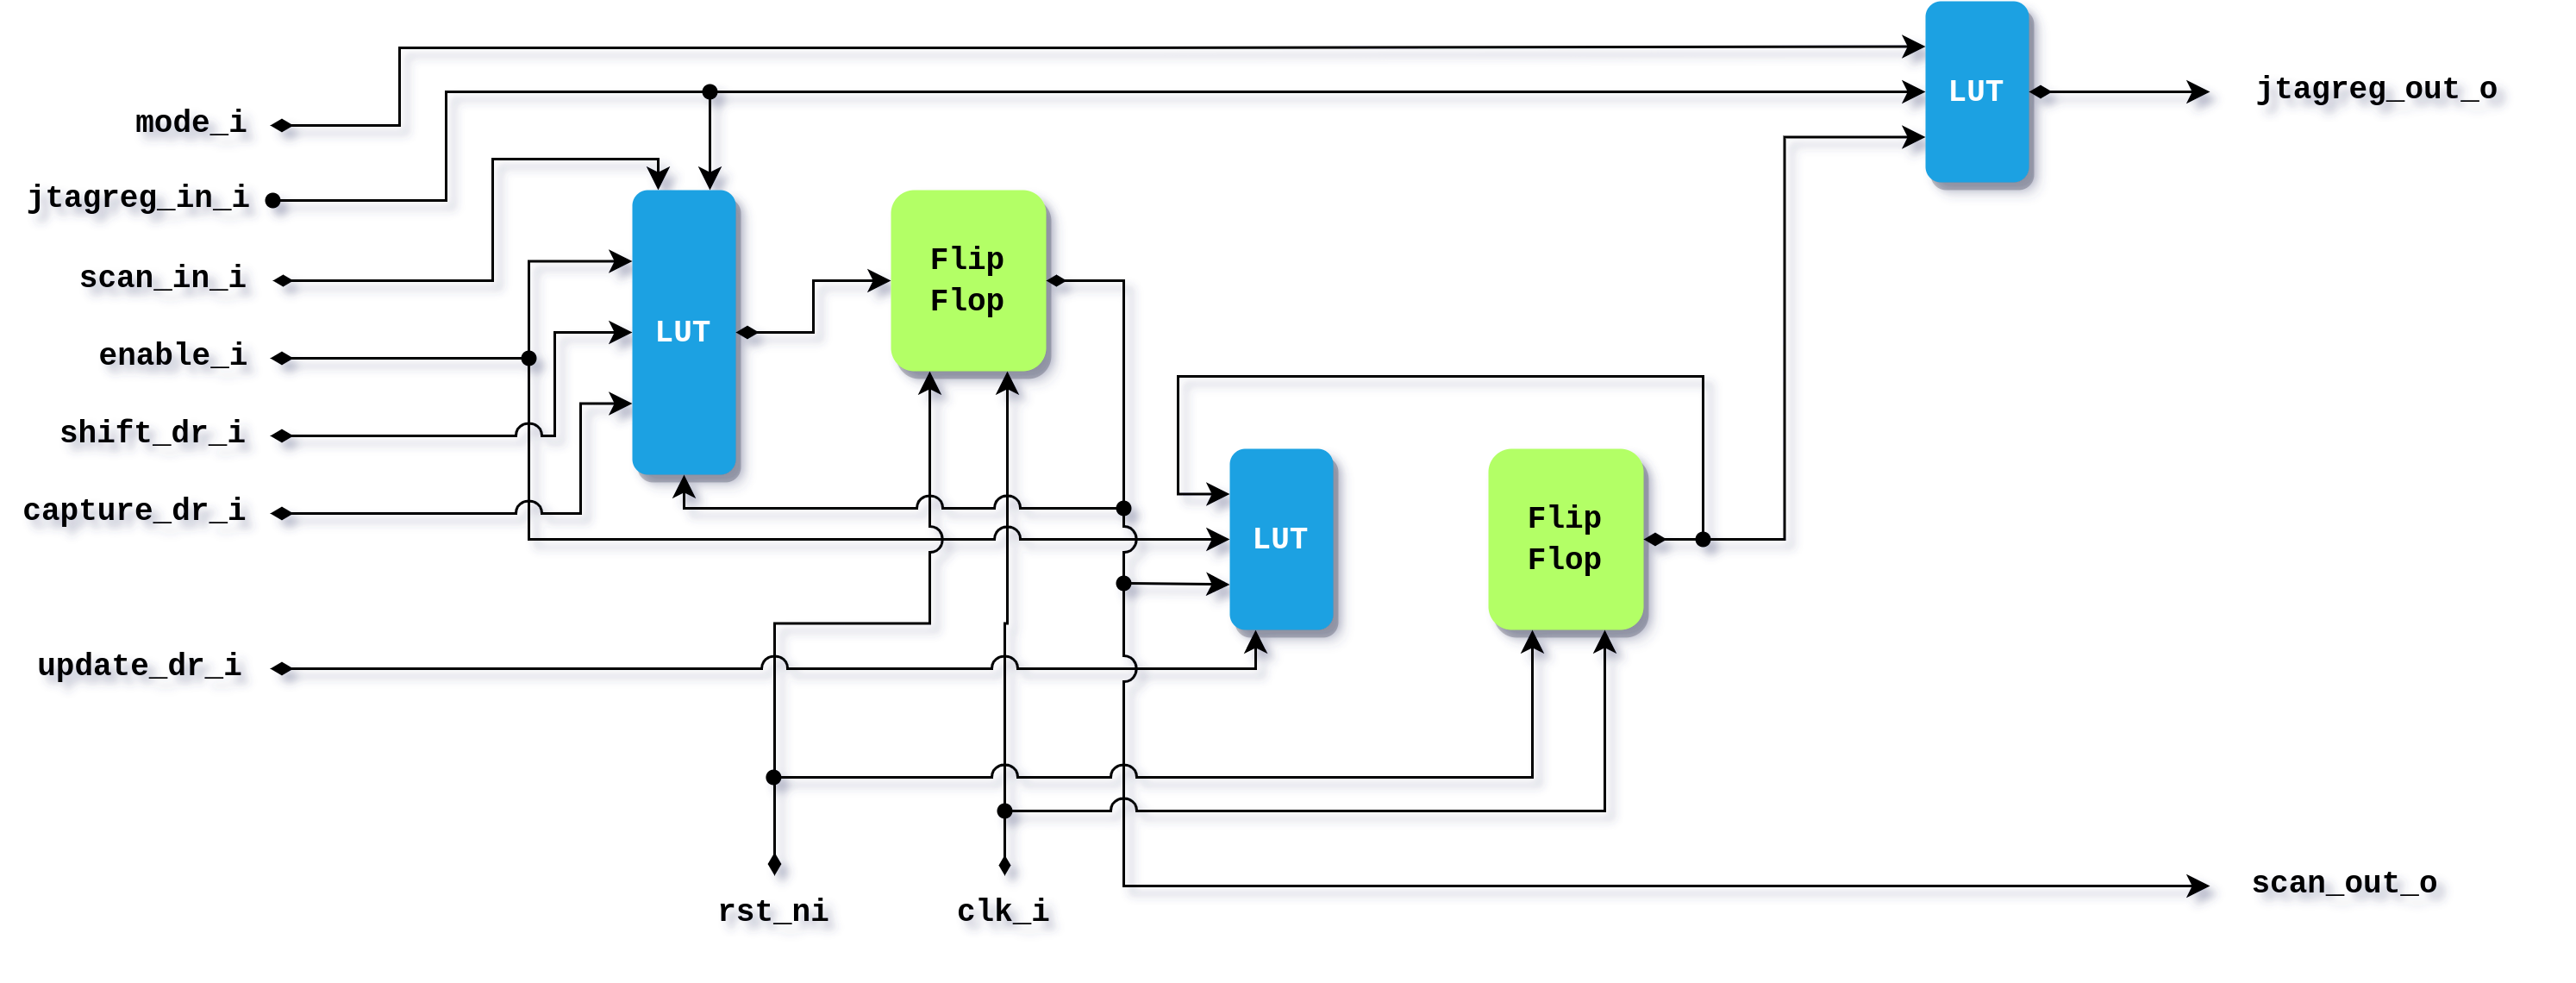
\includegraphics[scale=0.17]{jtag_bscell.png}
	\caption{Schematic of the boundary scan cell.}
	\label{fig:jtag_fsm}
\end{figure}

\subsection{AXI-Master Interface}

The table below shows the AXI4 Full interface signals as implemented in the IP.

\begin{table}[h]
\centering
	\resizebox{9cm}{!}{%
		\begin{tabular}{|l|l|l|}
			\hline
			\textbf{Signal Name} & \textbf{Bits} & \textbf{Implementation in the IP}   \\ \hline
			AW_ID       & Gemini        & LUTS= ??             \\ \hline
			Maximum Resource       & Gemini        & LUTS= ??             \\ \hline
		\end{tabular}
	}
	\caption{Raptor Report}
	\label{tab:table-2}
\end{table}

\subsection{TAP Controller}
\begin{figure}[!ht]\centering % Using \begin{figure*} makes the figure take up the entire width of the page
	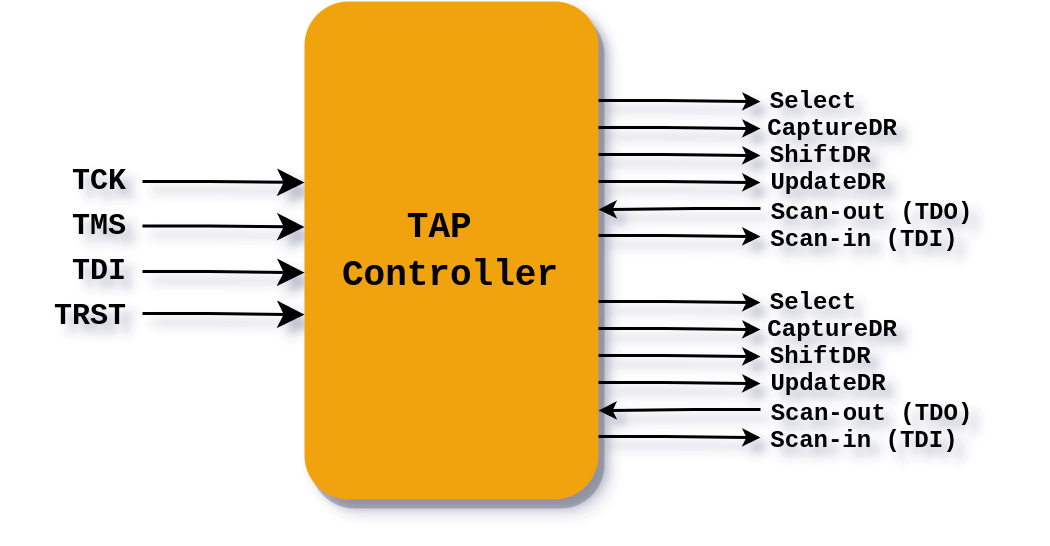
\includegraphics[scale=0.4]{jtag_tap.png}
	\caption{TAP Controller block diagram.}
	\label{fig:tap_controller}
\end{figure}

\subsection{TAP Controller State Machine}
\begin{figure}[!ht]\centering % Using \begin{figure*} makes the figure take up the entire width of the page
	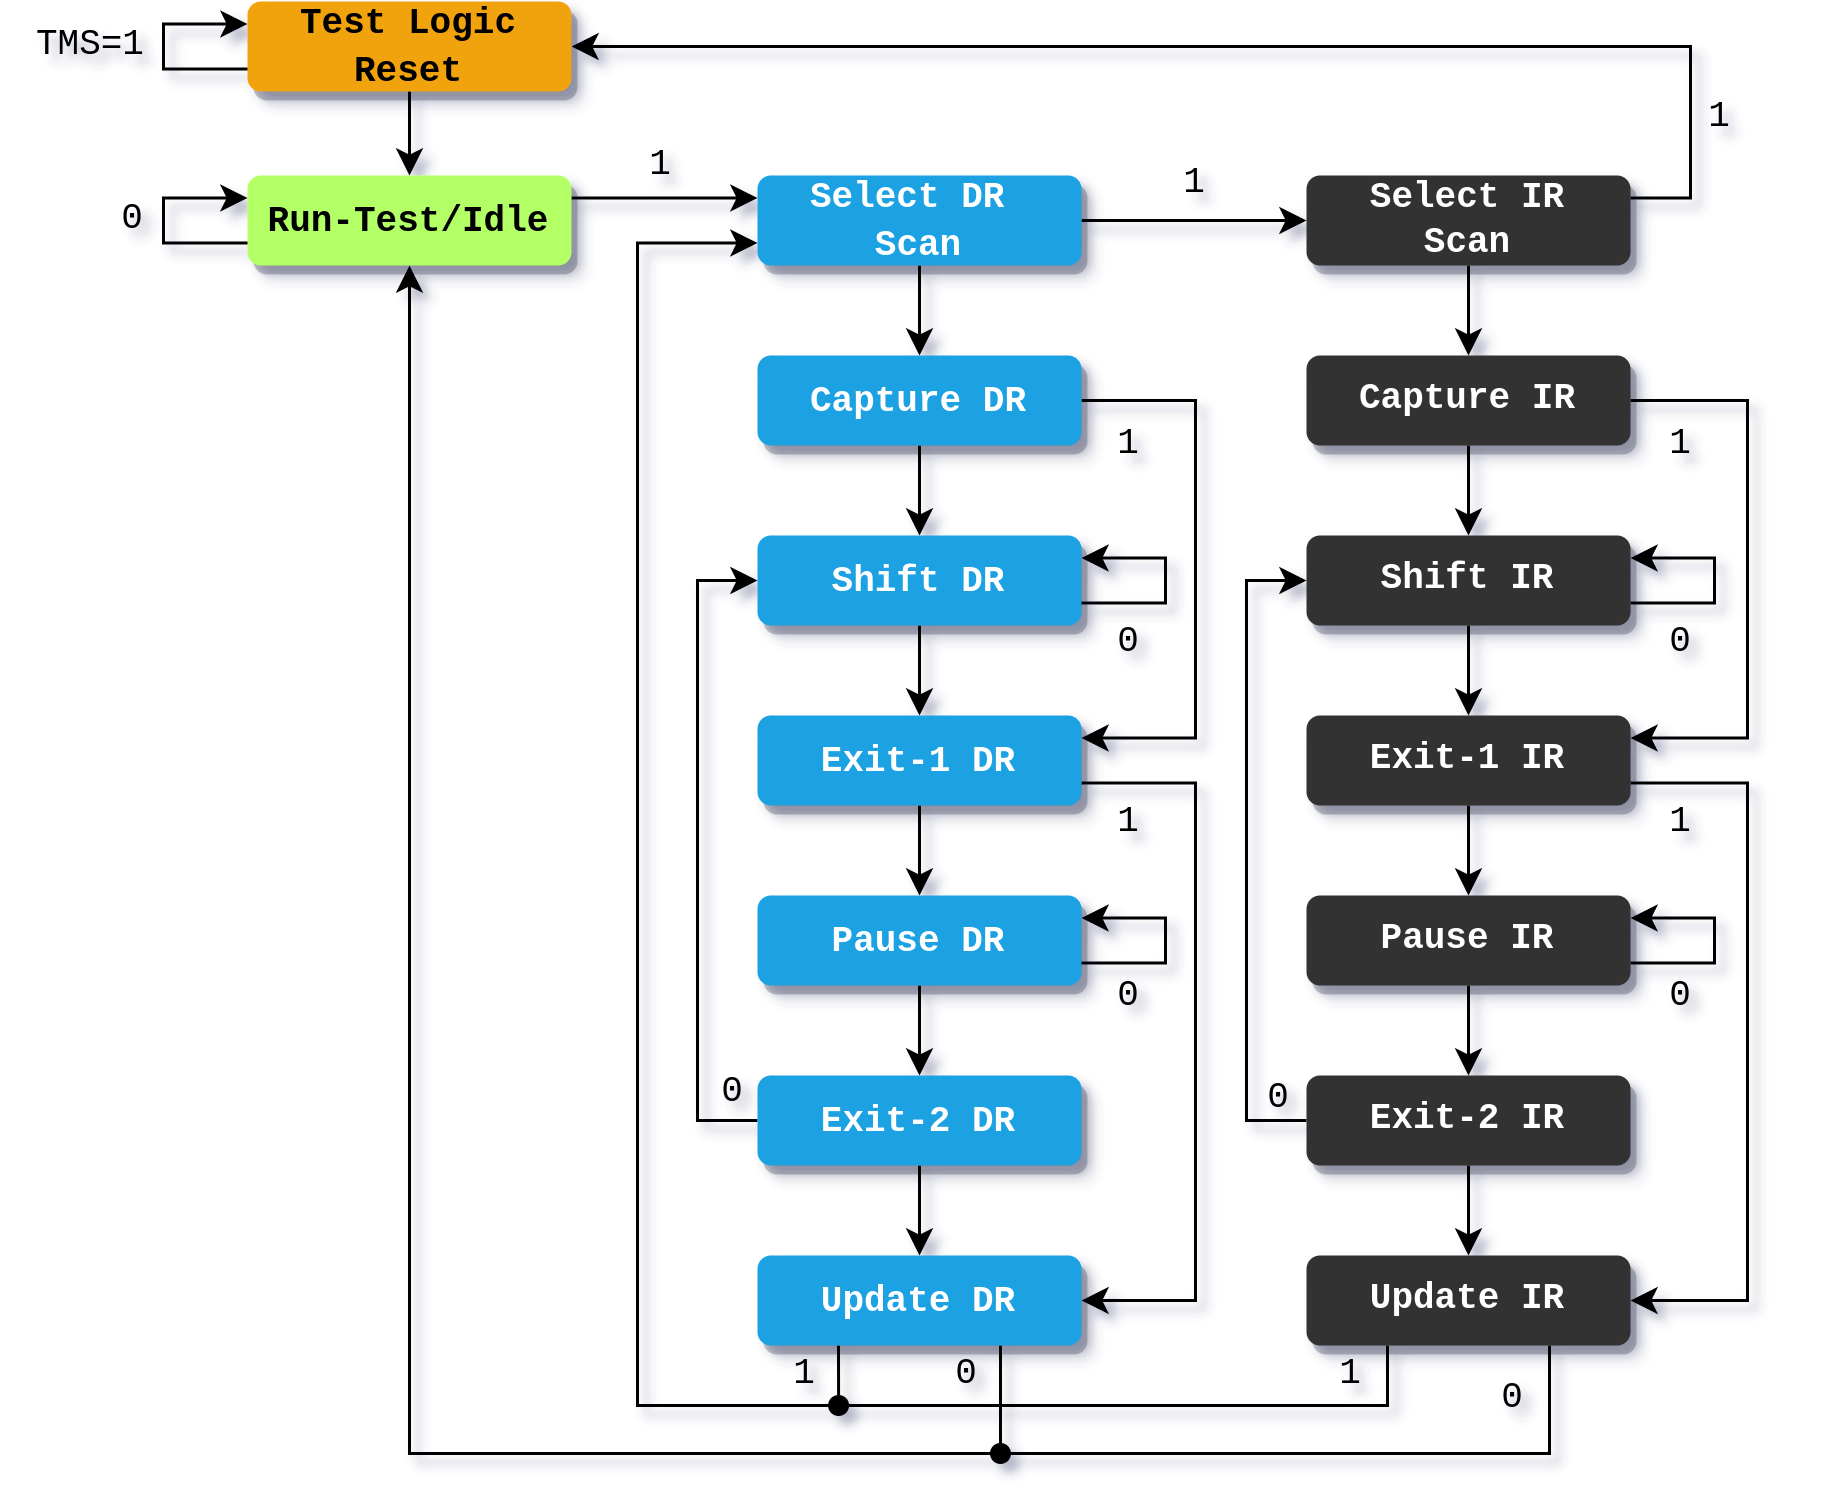
\includegraphics[scale=0.22]{jtag_fsm.png}
	\caption{FSM of JTAG TAP controller.}
	\label{fig:jtag_fsm}
\end{figure}

\subsection{High Level Block Design}
\begin{figure}[!ht]\centering % Using \begin{figure*} makes the figure take up the entire width of the page
	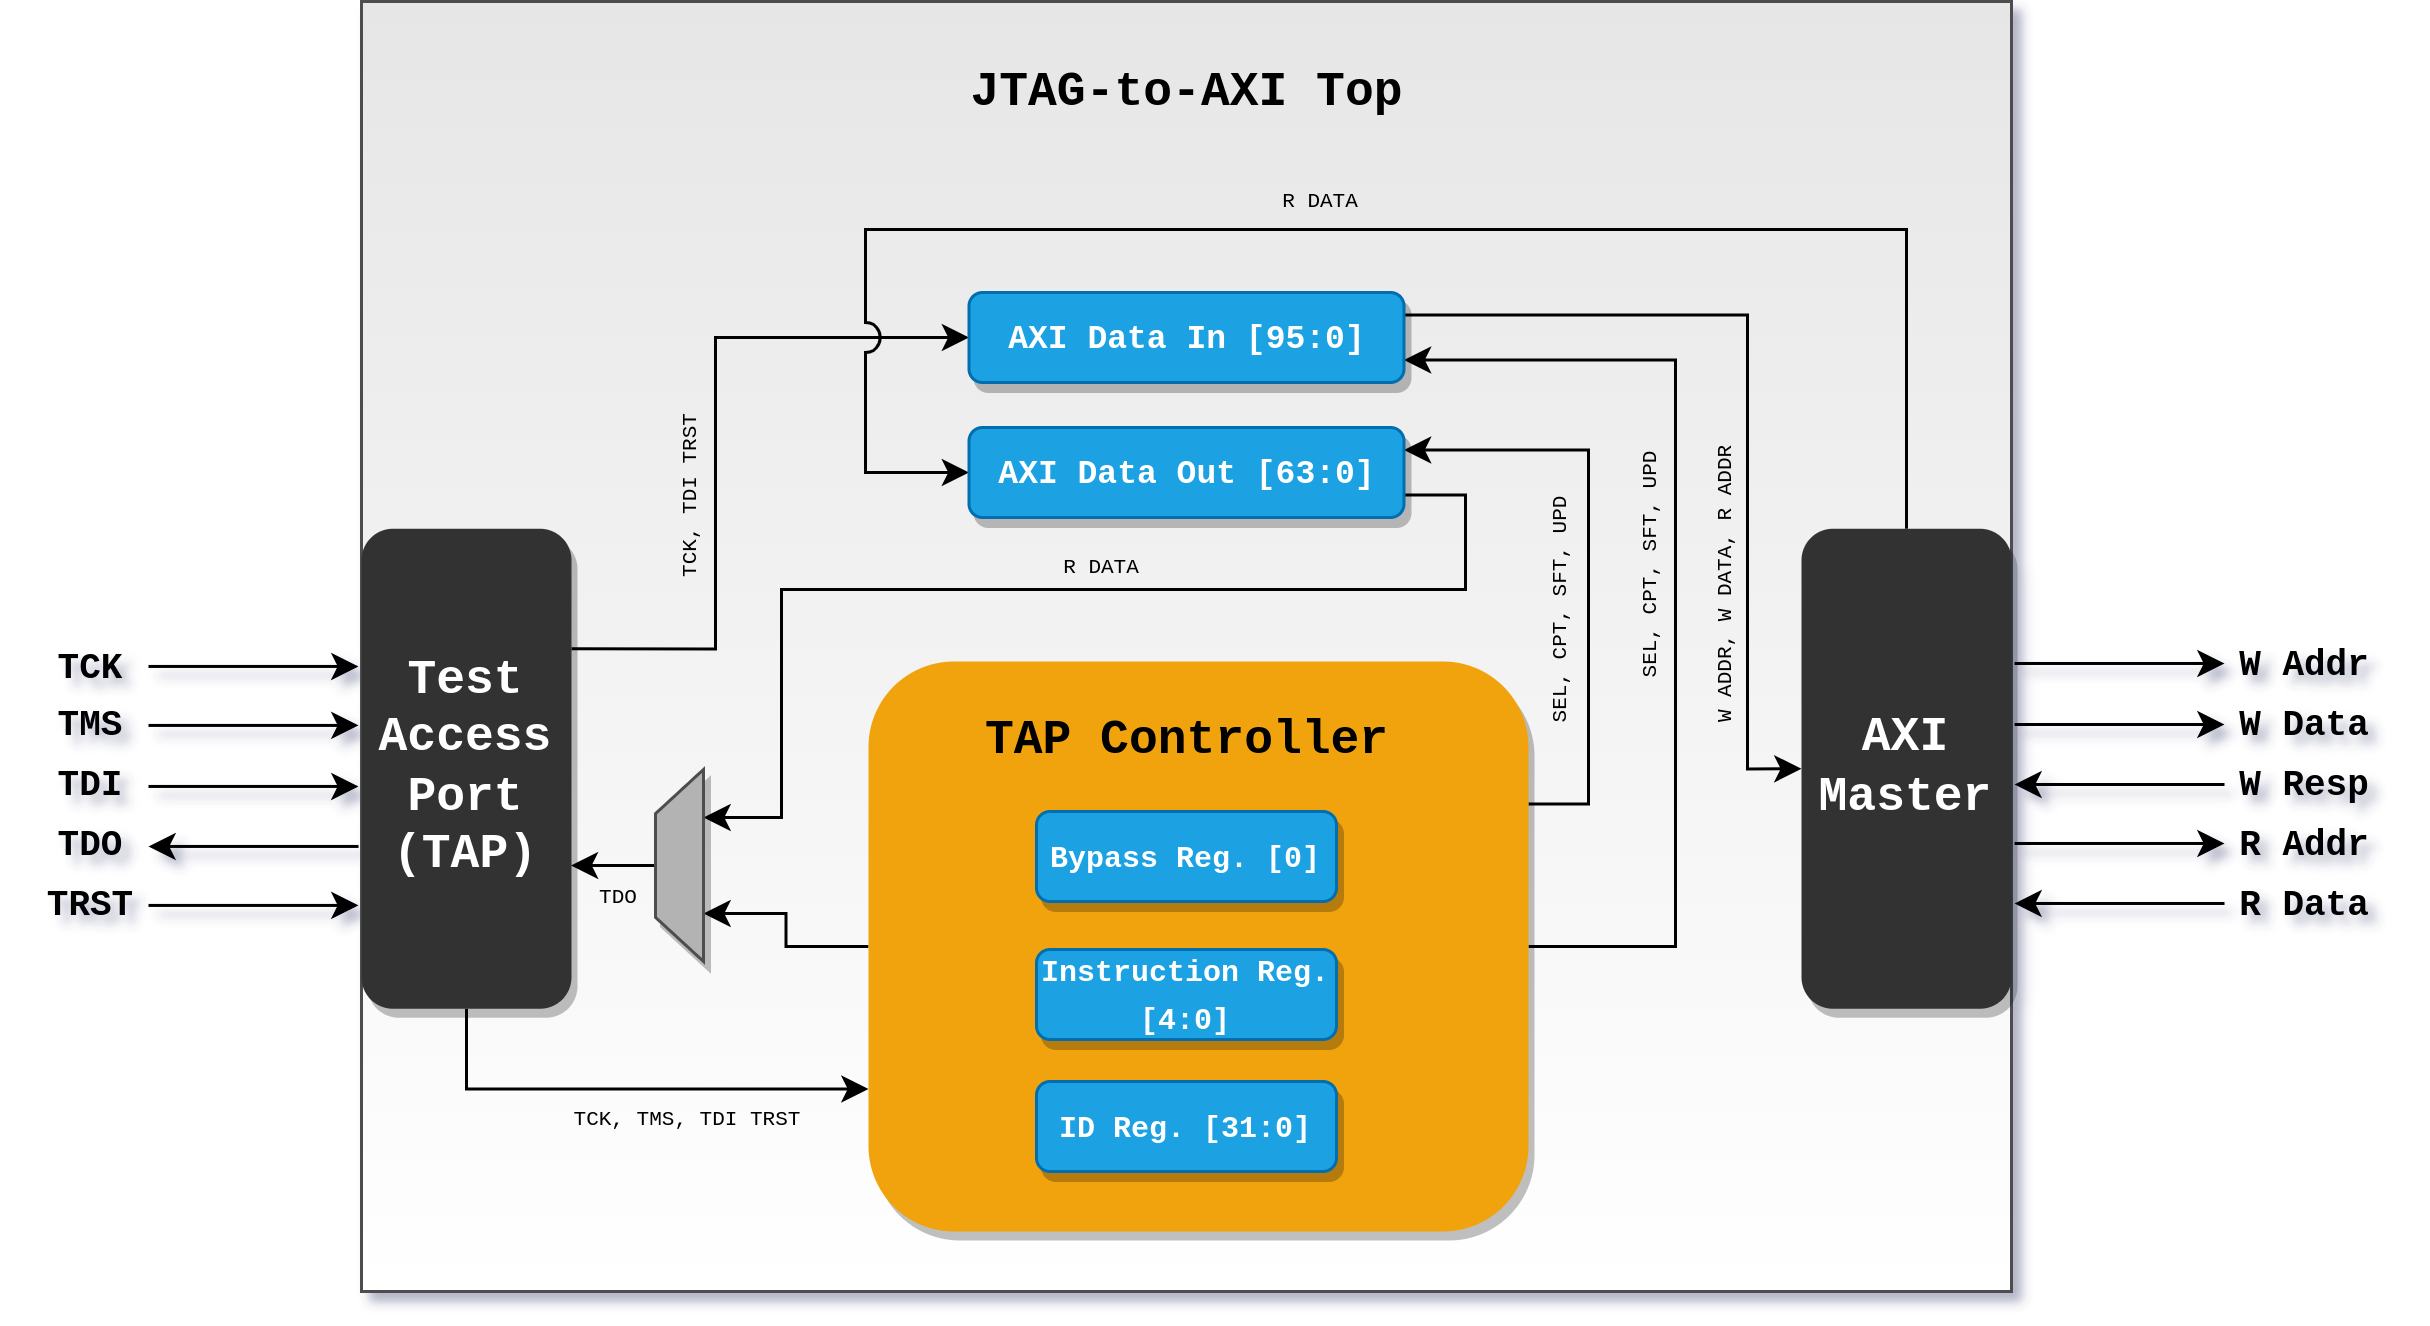
\includegraphics[scale=0.2]{jtag_bd.png}
	\caption{High-level block diagram of JTAG-to-AXI top module.}
	\label{fig:high_level_bd}
\end{figure}

% \subsection{Resource utilization}
% \FloatBarrier
% \begin{table}[h]
% 	\resizebox{\textwidth}{!}{%
% 		\begin{tabular}{|l|l|l|l|}
% 			\hline
% 			\textbf{Configuration} & \textbf{FPGA} & \textbf{Resources}                       & \textbf{Description}                            \\ \hline
% 			Minimum Resource       & GEMINI        & LUTS= ?? , FLOPS = ??, BRAM = ?? DSP =?? & configured to use minimum resources of the fpga \\ & & & i.e. number of probe = 1, data depth  = 1024, edge trigger \\ & & &  or no trigger, no trigger input or output, probe width 1                    \\ \hline
% 			Maximum Resource       & GEMINI        & LUTS= ?? , FLOPS = ??, BRAM = ?? DSP =?? & configured to use maximum resources of the fpga \\ & & & i.e. number of probe = 128, data depth  =  2\textasciicircum{}15 , edge trigger \\ & & &   or no trigger, no trigger input or output, probe width = 32            \\ \hline
% 		\end{tabular}%
% 	}
% 	\caption{Raptor Report}
% 	\label{tab:my-table}
% \end{table}
\FloatBarrier
\vfill
\newpage
%------------------------------------------------

\section {Revision History}

\begin{table}[hbt!]
	%\caption{Interrupt ports}
	%	\centering
	\begin{tabular}{|l|l|l|}
		\toprule
		%		\multicolumn{3}{c}{Name} \\
		%		\cmidrule(r){1-3}
		Date          & Version & Revisions                                              \\
		%\midrule
		\hline \text{October 10, 2022} & 0.01    & Initial version of the design / specification document
		\tabularnewline\hline
		%\bottomrule
	\end{tabular}

	%\label{tab:}
\end{table}
%----------------------------------------------------------------------------------------
%	REFERENCE LIST
%----------------------------------------------------------------------------------------

\phantomsection
\bibliographystyle{unsrt}
\bibliography{sample.bib}

%----------------------------------------------------------------------------------------

\end{document}
